\documentclass[11pt,a4paper,spanish]{article}

%--- Paquete para ajustar los margenes
\usepackage[a4paper,left=3cm,right=2cm]{geometry}
%\usepackage{anysize} 
%\marginsize{3cm}{3cm}{2cm}{2cm} 

%--- Paquete para escribir en español.
\usepackage[spanish, activeacute]{babel}

%--- Paquetes para meter los caracteres acencuados en Linux las dos codificaciones.
\usepackage[utf8]{inputenc}
%\usepackage[latin1]{inputenc}
%--- Paquete para meter los caracteres acentuados en Windows.
%\usepackage[ansinew]{inputenc}

%--- Paquete para insertar imagenes.
\usepackage[pdftex]{color, graphicx}

%--- Paquete para los hipervinculos, cambio los colores horribles por defecto.
\usepackage[pdftex, colorlinks=true, urlcolor=blue, linkcolor=blue]{hyperref}

%--- Paquete para meteter las figuras exactamente donde yo quiero en un entorno
%---- figure aunque queden feas.
\usepackage{float}
%--- Paquete para el lo que escribo en el .tex salga igual en .pdf aunque quede feo.
\usepackage{verbatim}

%--- Paquete para usar letras que se usan en matematica.
\usepackage{amsfonts}
%--- Paquete para escribir expresiones matematicas.
\usepackage{amsmath}

\usepackage[table]{xcolor}

\usepackage[showlabels,sections,floats,textmath,displaymath]{preview}


% Esto sirve para incluir palabras claves
\newcommand{\keywords}[1]{\par\vskip11pt\hskip10pt\noindent{\small{\bf Palabras Claves\/}: #1}}
\newtheorem{proposition}{Proposición}
\providecommand{\abs}[1]{\lvert#1\rvert}
\providecommand{\norm}[1]{\lVert#1\rVert}

\newcommand{\real}{\mathbb{R}}


%-------------- TP ------------------------------------------------------------
\begin{document}

%-------------- Caratula-------------------------------------------------------
\thispagestyle{empty}
\begin{center}


\includegraphics[width=0.18\textwidth]{escudo.png} \\[2em]

\begin{bf}
  Sistemas Operativos \\
  Departamento de Computación \\
  Facultad de Ciencias Exactas y Naturales \\
  Universidad de Buenos Aires \\[1.5em]
\end{bf}

{\large \bf Trabajo Práctico 1: \\ Scheduling} \\[2em]

\begin{tabular}{ll}
  Adrian Vinocur & \href{mailto:adrian.vinocur@gmail.com}{adrian.vinocur@gmail.com} \\
  Alejandro Albertini & \href{mailto:ale.dc@hotmail.com}{ale.dc@hotmail.com} \\
  Raul Brum & \href{mailto:brumraul@gmail.com}{brumraul@gmail.com} \\[2em]
\end{tabular}


\begin{abstract}
  En este trabajo estudiaremos el problema de planificar (scheduling) la ejecucición de tareas. Analizaremos de manera experimental algunos de los algoritmos clasicos como FCFS, Round Robin. Además analizaremos otros que utilizan prioridades para resolver el problema de planificación en tiempo real como RM (Rate Monotonic) y EDF (Earlier Deadline First).

\end{abstract}

\keywords{Scheluder, Scheduling, FCFS, Round Robin, RM, Rate Monotonic, EDF, Earlier Deadline First, Quantum}

\end{center}


%-------------- Tabla de contenido  -------------------------------------------
\newpage
\tableofcontents

%-------------- Cuerpo  -------------------------------------------------------

\section{Introducción}

En el presente trabajo nos proponemos a implementar la lógica de varios planificadores de tareas.

Nuestro trabajo consistir\'a en implementar, utilizando las estructuras provistas por la c\'atedra, ciertos algoritmos de \textit{scheduling} en lenguaje c++. Realizaremos experimentos empíricos e intentaremos hallar el \textit{quantum} \'optimo para el algoritmo de \textit{Round Robin}, con respecto a varias m\'etricas. Estas m\'etricas podr\'ian implicar criterios contradictorios, por lo que el objetivo ser\'a encontrar un balance adecuado entre ellas.

Además analizaremos un paper sobre scheduling basados en prioridades para procesos en tiempo real con ciertos requerimientos de deadlines obligatorios. Implementaremos estos últimos y buscaremos ejemplos para ilustrar el comportamiento de estos.

El trabajo se encuentra dividido en 10 ejercicios cuya meta de estos es abarcar lo anteriormente comentado. Se decidio omitir una secci\'on resultados agregando los gráficos directamente en el desarrollo. Lo que se busca con esta estructuración del informe es mantener cada ejercicio con explicaciones y gr\'aficos juntos para comodidad del lector.


\section{Desarrollo}

\subsection{Ejercicio 1}

La tarea TaskConsola simula una tarea interactiva en donde realiza $n$ llamadas bloqueantes de duración de tiempo aleatoria entre $bmin$ y $bmax$. Se pasa por parámetro la variable pid, y un vector con las variables $n$, $bmin$ y $bmax$, en ese orden. \\

Se coloca un ciclo for donde se itera $n$ veces y por cada iteración se produce una llamada bloqueante de tiempo aleatorio entre $bmin$ y $bmax$, para un respectivo pid. Ese número aleatorio se arma usando una función llamada ''$rand()$'' que genera un número aleatorio cualquiera y lo que hacemos es dividirlo por la diferencia entre $bmax$ y $bmin + 1$, quedándonos con el resto y a eso sumarle $bmin$ para acomodarlo entre el rango $[bmin, bmax]$. \\


\subsection{Ejercicio 2}

En este ejercicio escribimos un lote de 3 tareas con 1 intensiva de cpu y 2 taskConsola. 
El objetivo es ver un ejemplo interesante donde el algoritmo FCFS no tiene un buen rendimiento,
especialmente para procesadores de un núcleo. \\

\noindent
A continuación mostraremos el lote de tareas elegido:
\verbatiminput{graficos/corrida1_eje2.tsk}

Las 3 tareas llegan en el mismo instante (en el instante 1), la primer taskConsola produce una sola llamada bloqueante pero entre 15 y 20 ticks de reloj, la segunda taskConsola ejecuta 6 llamadas bloqueantes pero cada una entre 1 y 2 ticks de reloj y la tarea CPU utiliza 5 ticks de reloj. \\

Básicamente tenemos:
\begin{itemize}
	\item 1 tarea CPU intensiva.
	\item 1 taskConsola que solo ejecuta una llamada bloqueante pero de muchos ciclos de reloj
	\item 1 taskConsola que ejecuta 6 llamadas bloqueantes pero de pocos ciclos de reloj.
\end{itemize}

\begin{center}
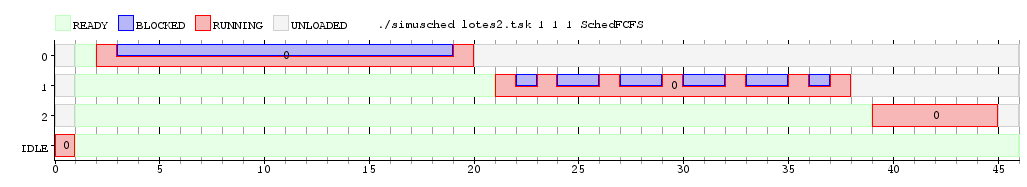
\includegraphics[scale=0.4]{graficos/imagen1.png}
\end{center}

Para un solo núcleo el problema que surge para la tarea CPU es que como el scheduler decidió que primero se ejecuten las dos taskConsola (a pesar de haber llegado las 3 al mismo tiempo), la tarea CPU tiene que esperar a que terminen las dos taskConsola para luego poder ejecutar solo 5 ciclos de reloj. \\

Si la tarea CPU hubiese llegado 1 solo ciclo de reloj antes se podría haber evitado la espera de las dos taskConsola y se hubiese ejecutado primero, reduciendo muchísimo su tiempo de espera. 
Otros de los puntos negativos es que la primer taskConsola tiene un tiempo de bloqueo muy grande lo que hace que se pierda mucho tiempo esperando que se resuelva y la segunda no tiene ningún bloqueo grande pero tiene 6 bloqueos de 1 o 2 ticks de reloj lo que hace que se pierda muchísimo tiempo con la cpu bloqueda esperando algún evento de entrada/salida por ejemplo. \\

\begin{center}
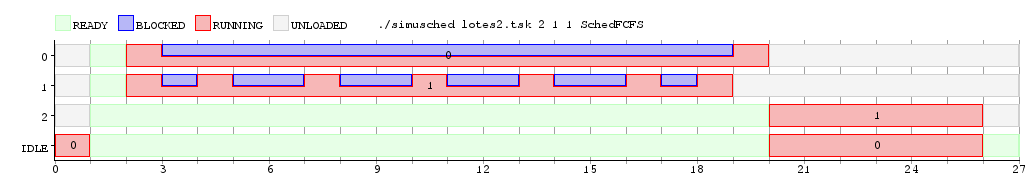
\includegraphics[scale=0.4]{graficos/imagen2.png}
\end{center}

En el caso en que tenemos 2 núcleos cambia mucho el panorama con respecto al de un núcleo.
Porque si bien otra vez la tareaCpu no es la elegida por el scheduler para comenzar, arrancan las dos taskConsola a la vez y la taskConsola2 de muchos ticks cortos no tiene que esperar a que termine de ejecutarse la primera, evitando así la taskConsola de un bloqueo grande, reduciendo muchísimo el tiempo de espera de la taskConsola2.\\

\begin{center}
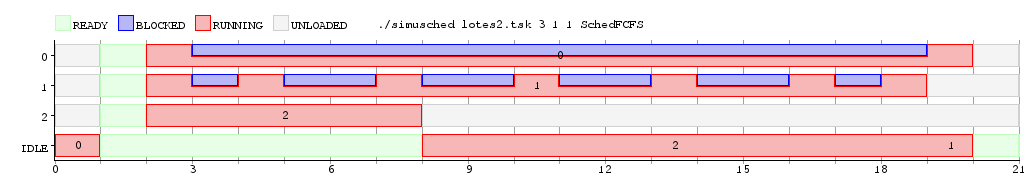
\includegraphics[scale=0.4]{graficos/imagen3.png}
\end{center}

Y el caso donde tenemos 3 núcleos es el ideal, ya que ninguna de las tareas tiene que esperar a que termine de ejecutarse la otra, todas empiezan a ejecutarse inmediatamente después de llegar al scheduler reduciendo drásticamente el tiempo de espera con respecto a los casos anteriores. \\

\noindent
Tick final de la ejecución de la última de las 3 tareas:
\begin{itemize}
	\item 1 núcleo: 45
	\item 2 núcleos: 26
	\item 3 núcleos: 20
\end{itemize}

\noindent
Mediciones del tiempo de espera para el algoritmo FCFS (en ticks unidades de tiempo):
\begin{itemize}
	\item Para 1 núcleo: 19,66
	\item Para 2 núcleos: 10,25 (52,14% con respecto al de 1 núcleo)
	\item Para 3 núcleos: 2,5 (12,72% con respecto al de 1 núcleo)
\end{itemize}

\noindent
Mediciones del turnaround para el algoritmo FCFS (en ticks unidades de tiempo):
\begin{itemize}
	\item Para 1 núcleo: 33,33
	\item Para 2 núcleos: 22 (66% con respecto al de 1 núcleo)
	\item Para 3 núcleos: 16 (48% con respecto al de 1 núcleo)
\end{itemize}


\subsection{Ejercicio 3}

\noindent

El algoritmo de scheduling de Round Robin\cite{silberschatz2009operating} (RR) está diseñado específicamente para cumplir con las necesidades de los sistemas de time-sharing. Es similar al scheduler FCFS, con la adición de desalojo (o preemption), lo cual le permite al sistema intercambiar los procesos en ejecución. Se define un quantum, que es una pequeña unidad de tiempo, por lo general de 10 a 100 milisegundos de longitud. La cola de ''listos'' (ready) se trata como una cola circular. El scheduler recorre la cola, asignando CPU a cada proceso por a los sumo 1 quantum de tiempo.
Para implementar RR, mantenemos la cola de ready como una cola FIFO de procesos. Los nuevos procesos son añadidos al final de la cola.  El CPU toma el primer proceso de la cola de ready, establece un timer para interrumpir luego de 1 quantum, y realiza el dispatch del proceso. \\

Luego pueden suceder una de dos cosas: 
\begin{itemize}
	\item El proceso utiliza CPU por menos que 1 quantum. En este caso el proceso mismo devolverá el CPU voluntariamente (ya sea porque terminó o porque se bloqueó). El scheduler procederá entonces con el siguiente proceso en la cola de ready. 
	\item El proceso continúa corriendo luego de 1 quantum. En este caso el timer se disparará, elevando una interrupción al sistema operativo. Entonces se realizará un cambio de contexto, en el cual el scheduler desalojará al proceso, que sera ubicado al final de la cola de ready, y procederá con el siguiente proceso en la mencionada cola.   
\end{itemize} 

En el algoritmo de Round Robin, ningún proceso es alocado en la CPU por más tiempo que un quantum (a menos que sea el único proceso que pueda ser ejecutado). Si un proceso excede el tiempo de un quantum en CPU, el mismo es desalojado y puesto nuevamente en la cola. Round Robin es por lo tanto un algoritmo con desalojo.
Si hay n procesos en la cola de ready y el quantum es q, entonces cada proceso recibe $1/n$ de tiempo de CPU en pedazos de a lo sumo q unidades de tiempo. Cada proceso esperará a lo sumo $(n-1)*q$ unidades de tiempo hasta su próximo quantum.   
La performance del algoritmo de Round Robin depende, como veremos más adelante, del tamaño del quantum. En un extremo, si el quantum es demasiado largo, se comporta como si fuera FCFS. En contraste, si el quantum es extremadamente corto, esto se denomina procesador compartido, y (en teoría) crea la apariencia de que cada uno de los $n$ procesos cuenta con su propio procesador corriendo a $1/n$ veces la velocidad real del procesador. \\

En esta sección nos propusimos simular un algoritmo de Round Robin que permita el intercambio entre procesadores. Esto significa, en este caso, que cada proceso recibirá el primer procesador libre que se encuentre, sin importar que sea o no el mismo procesador en el que se haya ejecutado previamente.
Para lograrlo, utilizamos las siguientes estructuras auxiliares: 
\begin{itemize}
	\item Una cola de ready, que contiene los PID de los procesos que están listos para ser ejecutados.
	\item Un mapa que almacena el proceso y el tiempo restante que cuenta para correr en cada core.
\end{itemize} 

El scheduler se inicializa con la tarea IDLE corriendo en cada core. El quantum asignado a la tarea IDLE es siempre cero, para que pueda ser desalojada a continuación por cualquier tarea ''real'' que requiera el uso de CPU. \\

Con cada tick del reloj, se evalúa qué hacer según el motivo del mismo: 
\begin{itemize}
	\item Si es un bloqueo, se remueve al proceso del CPU y el mismo renuncia a su quantum restante. El mismo será colocado de vuelta al final de la cola de ready cuando se reciba la señal de que se ha desbloqueado. Si hay un proceso disponible en la cola de ready, se le asignará ese core y se establecerá su tiempo disponible como el total del quantum. Caso contrario, se asignará un ciclo de ejecución en ese core a la tarea IDLE.
	\item Si el proceso ha finalizado, se remueve el proceso del CPU, y se procede al siguiente en la cola como  en el caso anterior.
	\item Si el proceso continúa en ejecución, se decrementa su tiempo disponible en CPU. Si ha excedido su quantum, será desalojado y puesto en el final de la cola de ready. Se retornará como proceso siguiente al primero de la cola, que podría ser el mismo proceso si no hubiera otro disponible.
\end{itemize}

\subsection{Ejercicio 4}

Se realizaron distintas corridas del algoritmo Round Robin, para ilustrar su comportamiento: \\

\noindent
Corrida 1:
\verbatiminput{graficos/corrida1_eje4.tsk}

\begin{center}
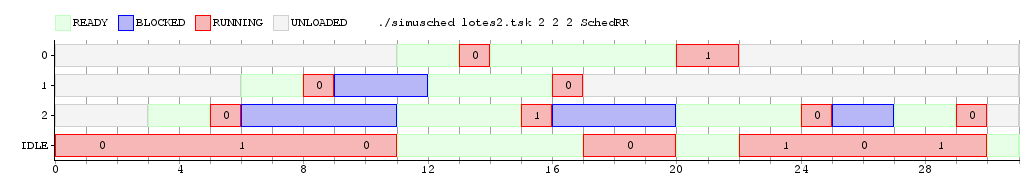
\includegraphics[scale=0.4]{graficos/rr_lotes2.png}
\end{center}

Como se puede observar, los procesos liberan el CPU al bloquearse. También se observa que los mismos cambian de procesador, como es el caso del 0 y el 2. Se nota en estos casos la penalidad de 2 ciclos por cambio de procesador (añadida a los 2 ciclos de cambio de contexto).  En este caso el quantum de ambos procesadores es 4. \\

\noindent
Corrida 2:
\verbatiminput{graficos/corrida2_eje4.tsk}

\begin{center}
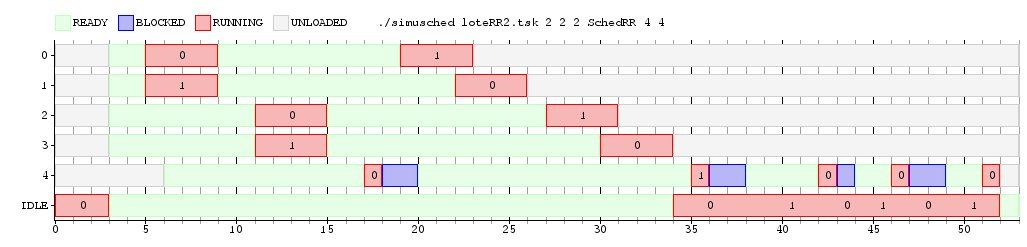
\includegraphics[scale=0.4]{graficos/rr2.png}
\end{center}

En este caso corren 4 tareas de cpu, y una de consola. El quantum es de 4 ciclos y se cuenta con 2 procesadores. Se puede observar como las tareas comparten el uso de CPU y son desalojadas al finalizar su quantum. También se observa que el scheduler, por simplicidad de implementación, no identifica en qué procesador estaba corriendo la tarea, causando una penalidad extra de cambio de procesador. También se observa que los tiempos de espera son bastante elevados en este caso.

\begin{center}
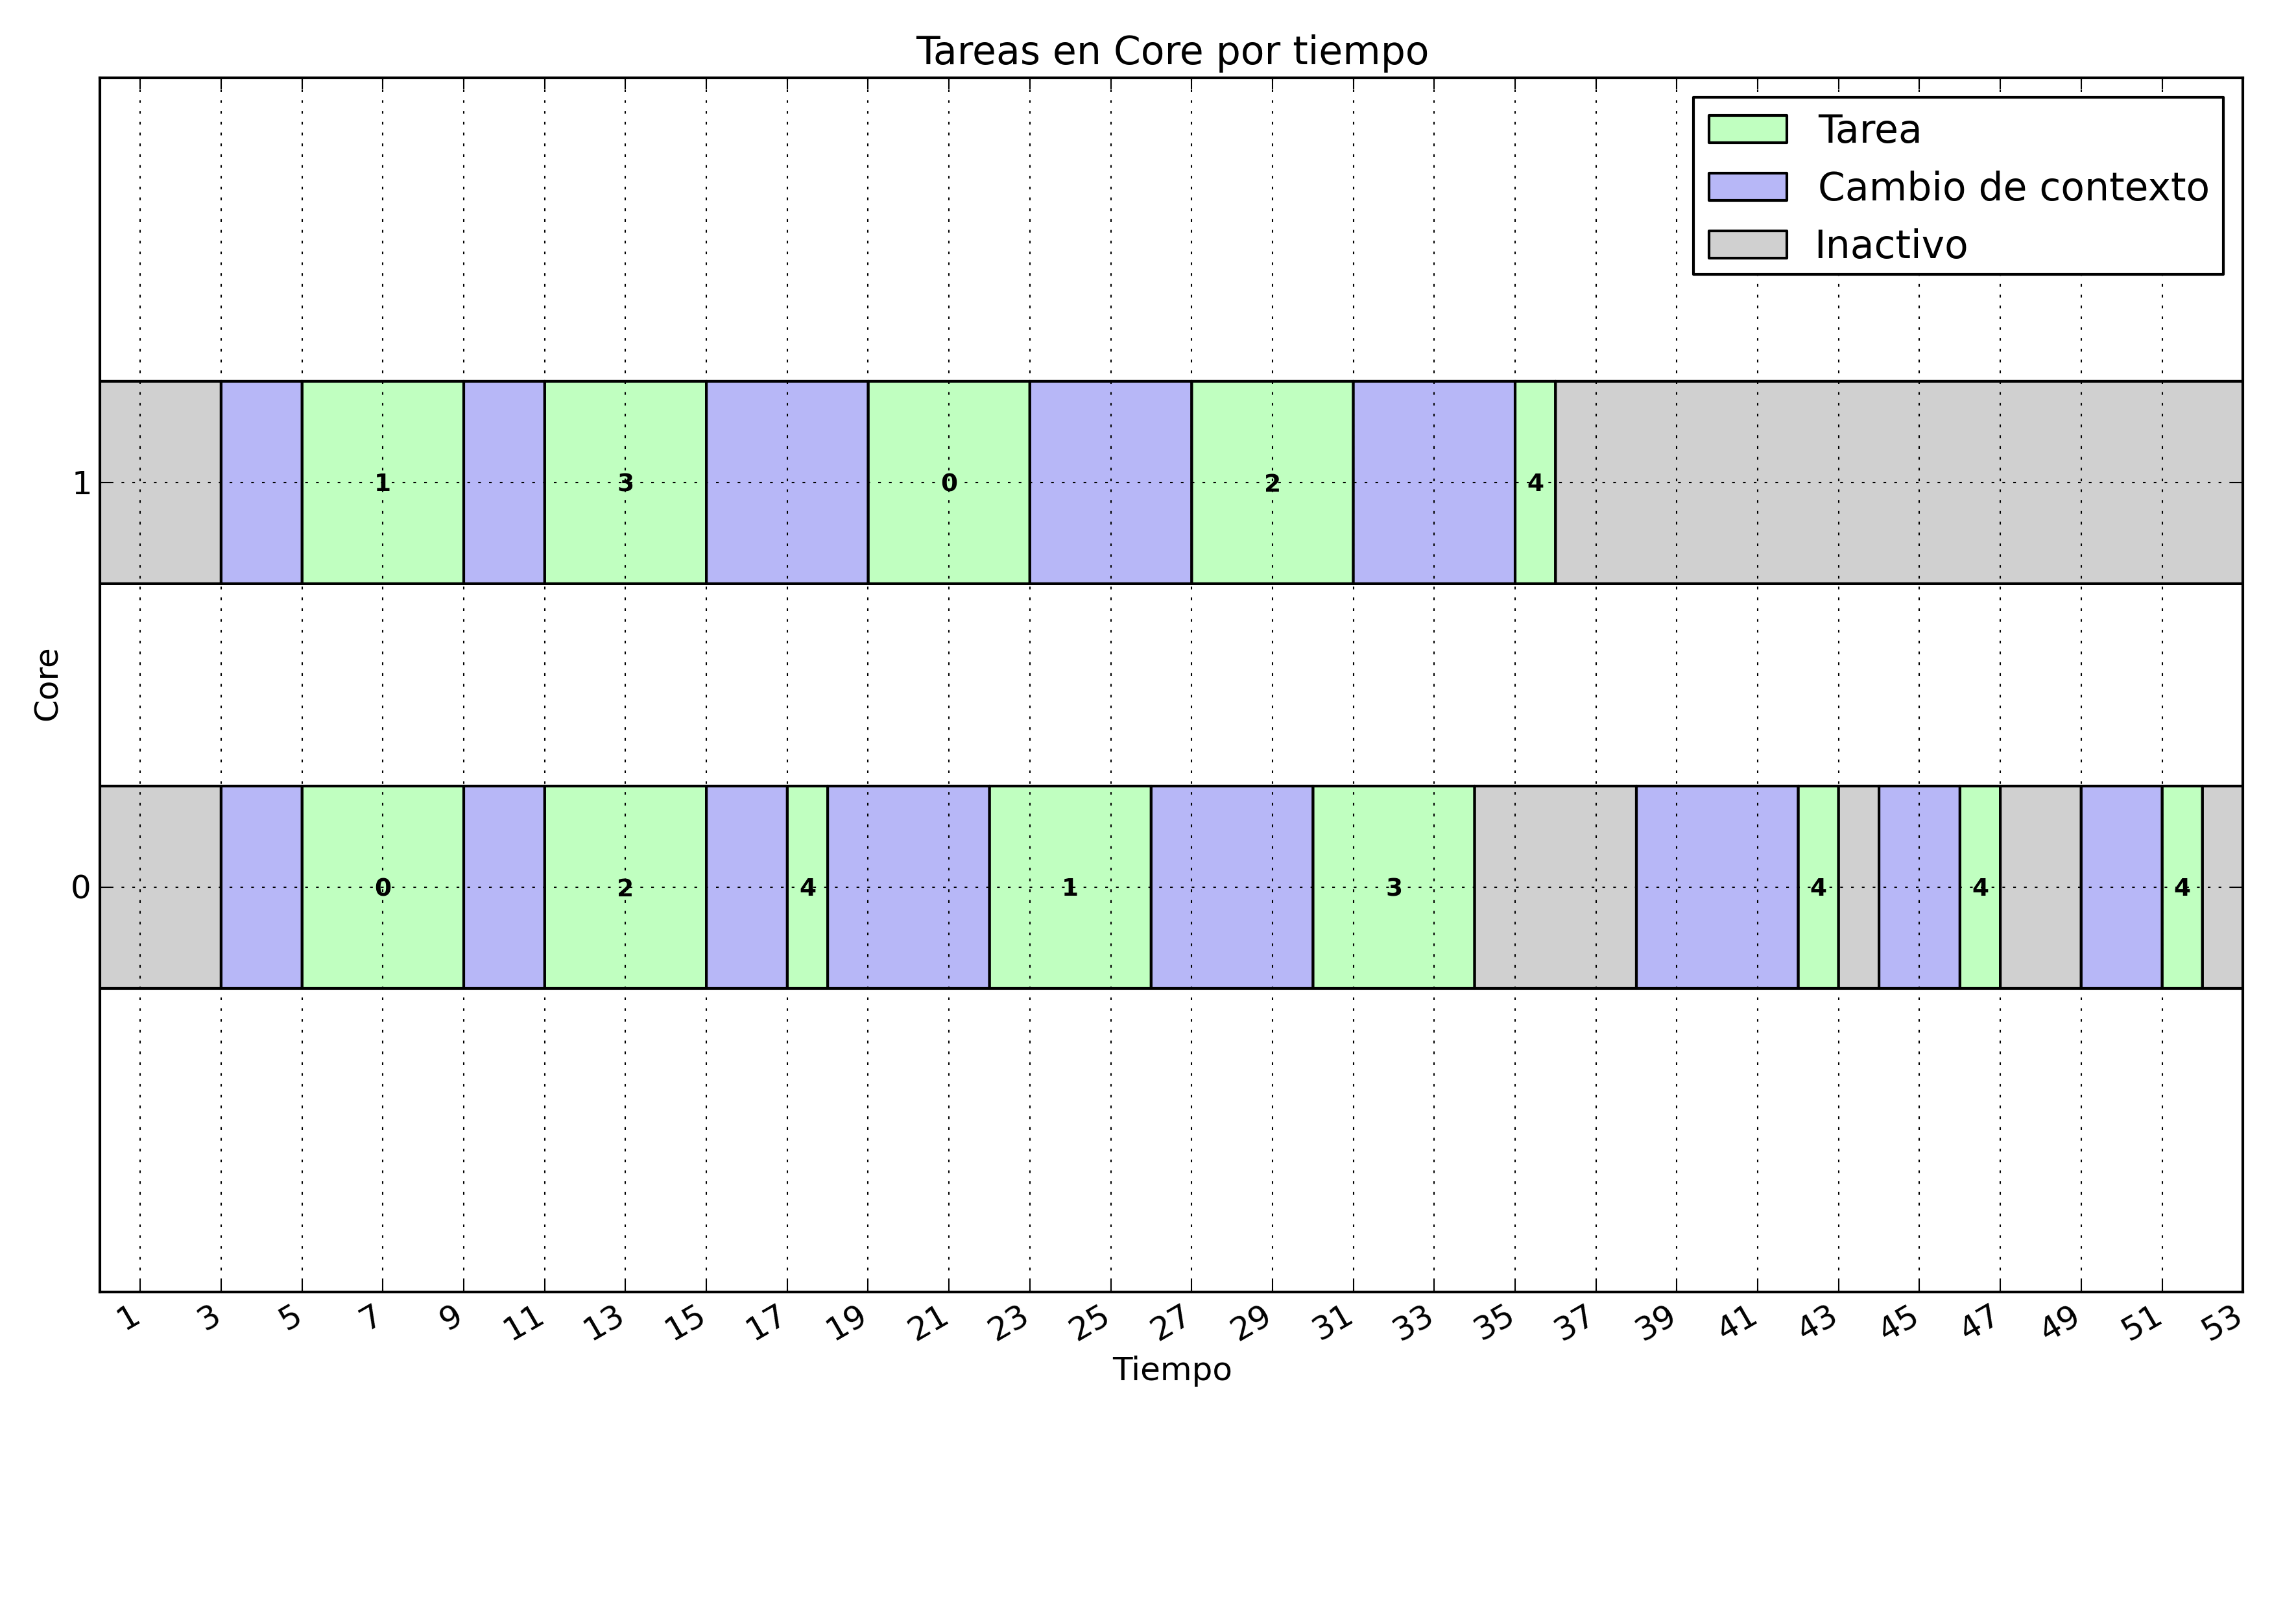
\includegraphics[scale=0.4]{graficos/out_cores_timeline.png}
\end{center}

En el gráfico anterior se observa más claramente que el algoritmo no es muy eficiente en este caso, ya que se está inviertiendo mucho tiempo en cambios de contexto (es casi lo mismo que el tiempo de ejecución real de las tareas).\\

\noindent
Corrida 3:
\verbatiminput{graficos/corrida3_eje4.tsk}

Se corrió en este caso con 2 cores y quantum 4. En este caso no se incluyeron tareas interactivas.

\begin{center}
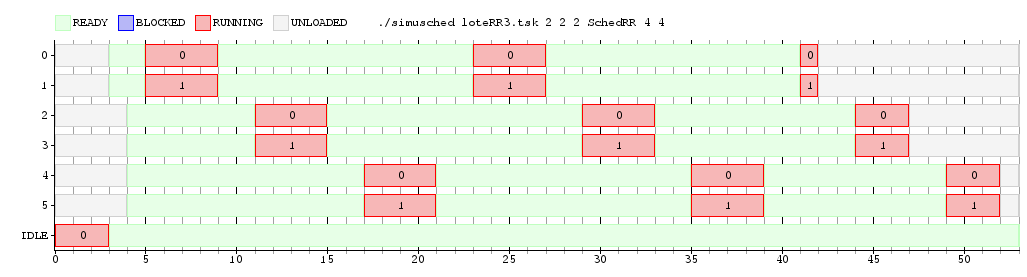
\includegraphics[scale=0.4]{graficos/rr_loteRR3.png}
\end{center}

Como se observa en los gráficos, este es un caso más ''feliz'', donde el costo de cambio de contexto es mucho menor, y la utilización del CPU es más eficiente (más uso en ejecución de las tareas que en cambios de contexto)

\begin{center}
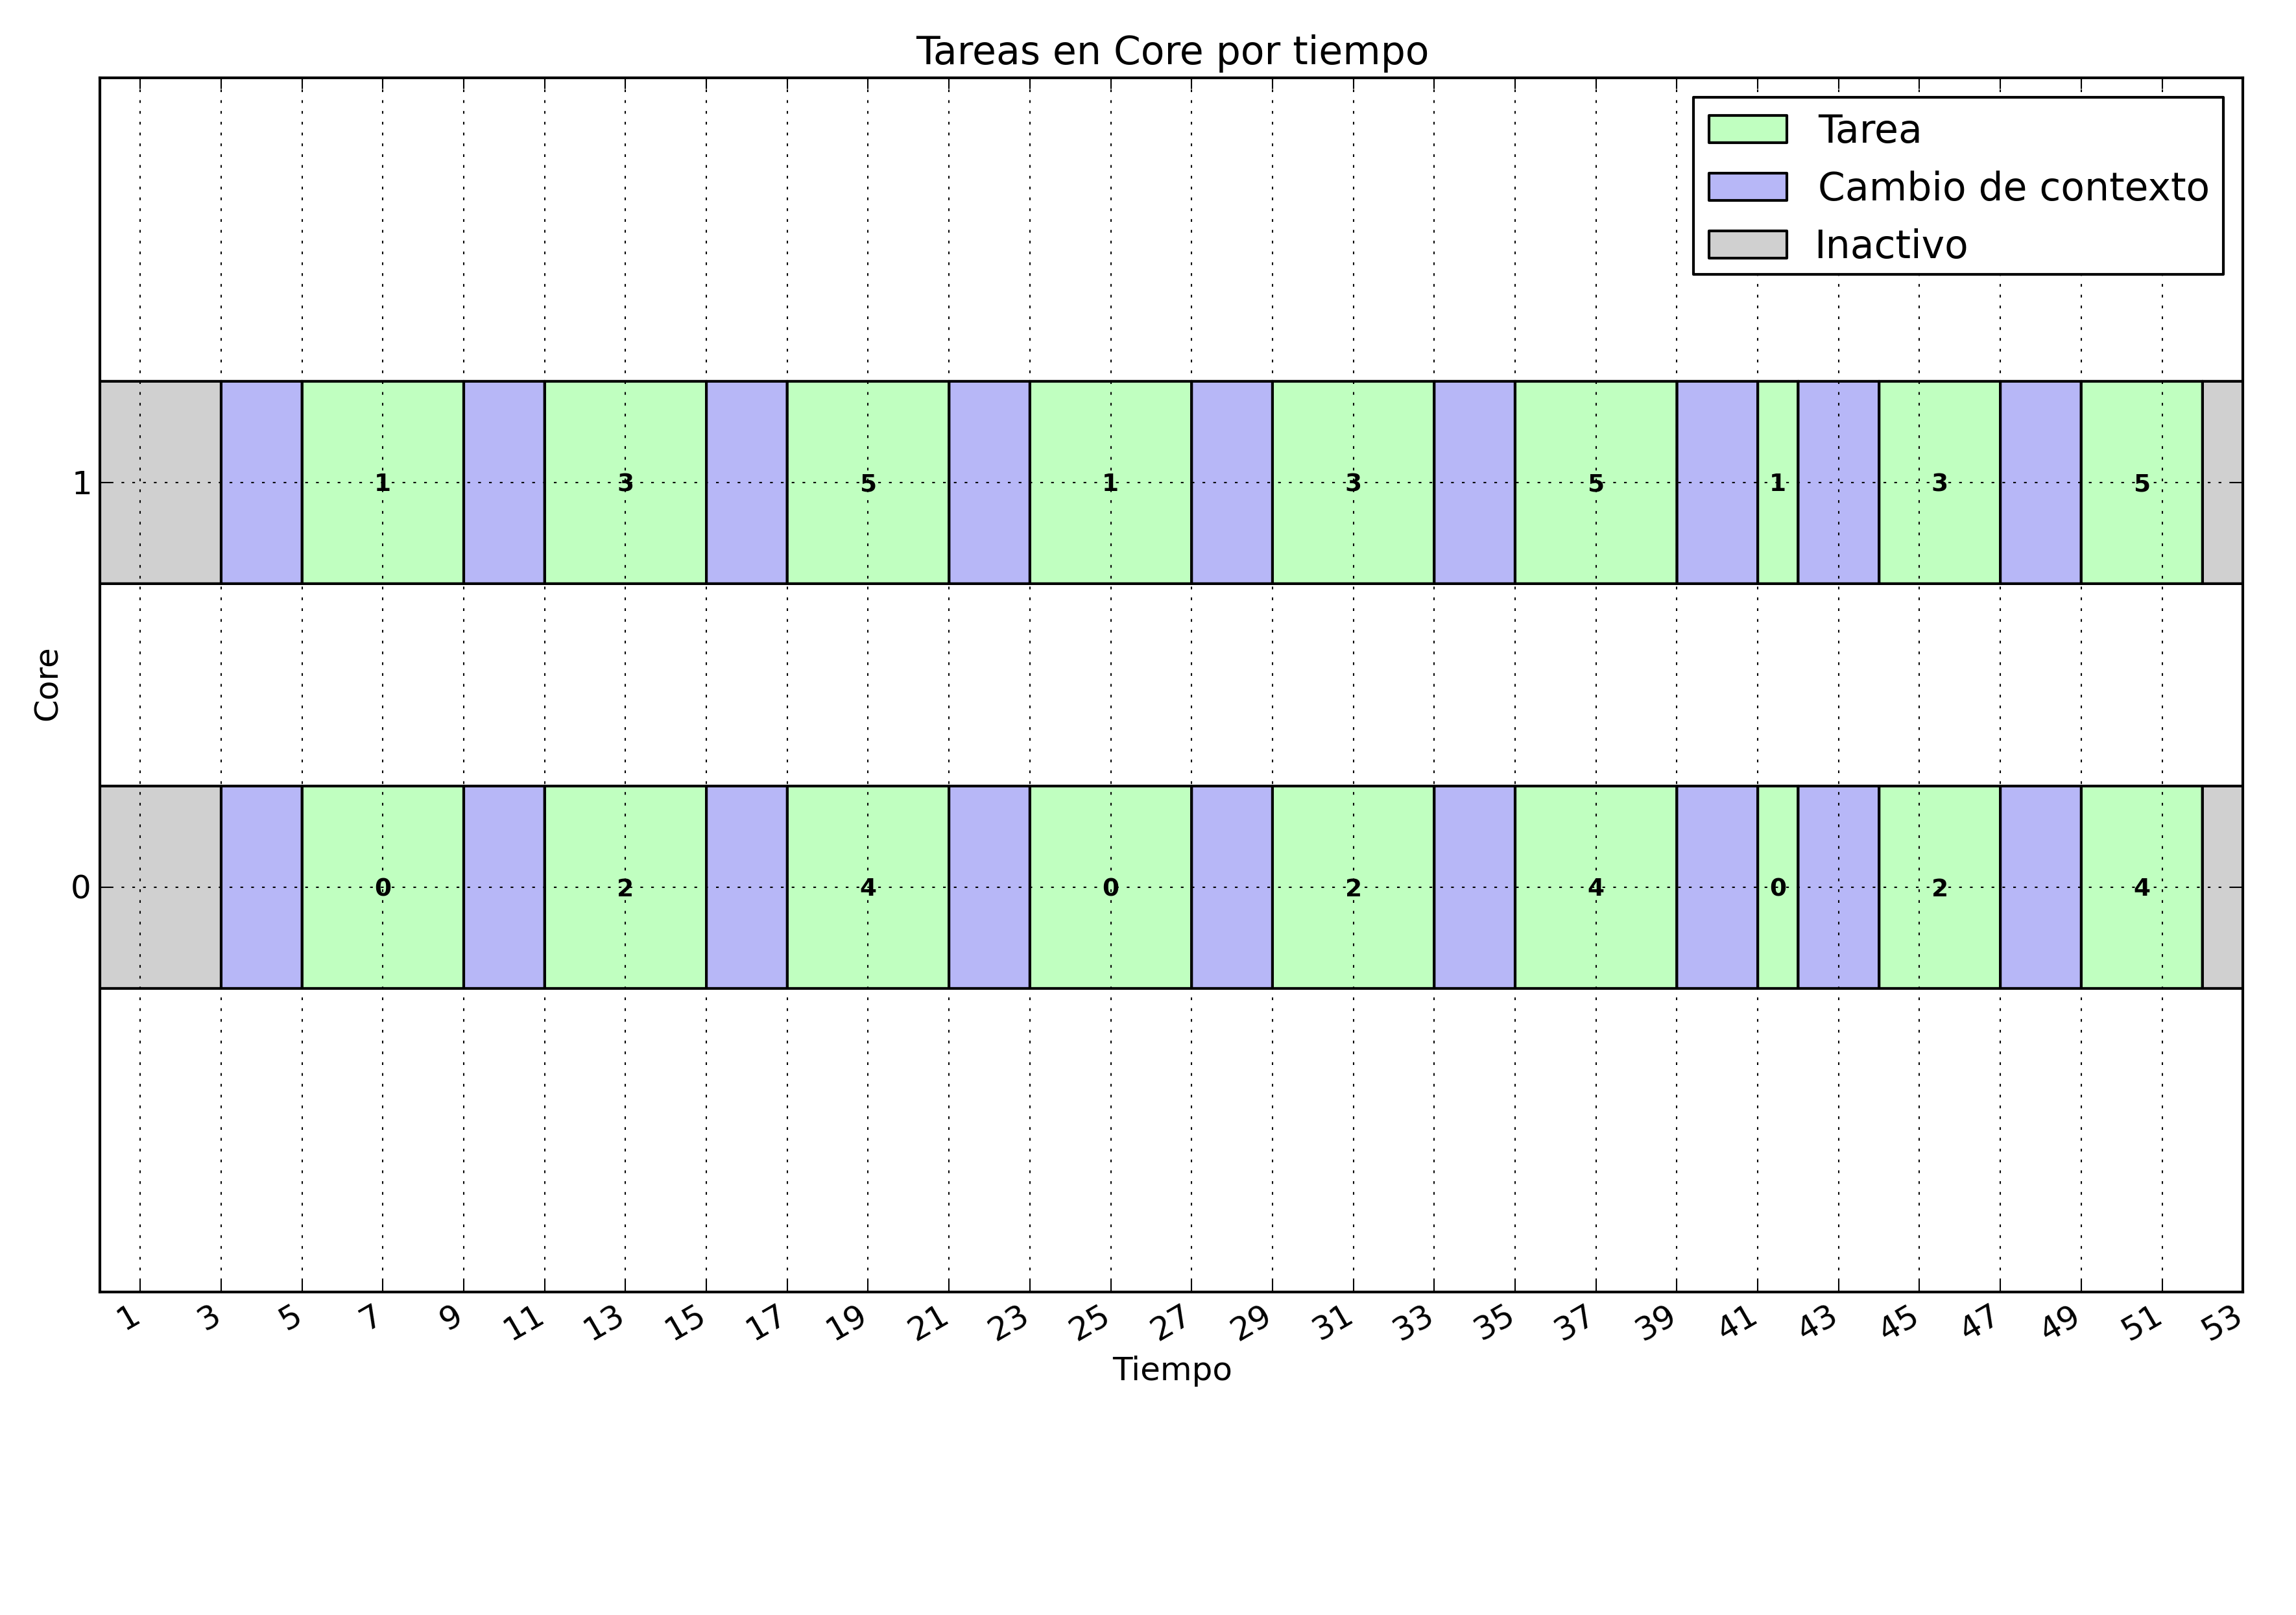
\includegraphics[scale=0.4]{graficos/out_cores_timeline1.png}
\end{center}


\subsection{Ejercicio 5}

El paper\cite{liu1973scheduling} se centra en la problemática de programar varias tareas con un solo procesador en un determinado contexto.
Dicho contexto establece que las tareas tiene que cumplir un deadline y hay que garantizar el cumplimiento de este. \\


Analizan únicamente schedulers que utilizan prioridades y que adminten desalajo (preemptive) de tareas (En particular RM, EDF y una versión mixta).\\


El algoritmo de la sección 7 lo introducen por las limitaciones de RM.\\


La cota que definen los autores para poder saber si un conjunto de N tareas es factible para N grande es aproximadamente de $ln(X)$ es decir un poco menos del 70\% de utilización de CPU.
Es decir si el conjunto de N tareas utiliza aprox menos de $ln(X)$ de tiempo de CPU entonces se puede programar con RM cumpliendo los deadlines, si no cumple esa cota dependerá del conjunto y los periodos de las tareas para determinar si es factible o no. \\


El algoritmo de EDF proporciona una cota de factibilidad mucho mejor, si y solo si es factible programar un conjunto de tareas si su procesamiento no supera el 100\% de uso de CPU.\\


Esta cota de factibilidad de programación de tareas que tiene EDF implica que un conjunto de tareas puede ser programado respetando deadlines por un scheduler si y solo si EDF es capaz de hacerlo.\\


El teorema 7 deduce la cota de factibilidad de programación de un conjunto de tareas utilizando el algoritmo EDF.\\

Consiste en analizar el consumo de CPU que asigna a cada tarea el algoritmo EDF en un rango de tiempo grande. Sumando estos tiempos se obtiene el uso total de CPU asignado a tareas en ese rango. \\

La demostración de que si las tareas usan más del 100\% no se pueden programar con un solo CPU es simple dado que vale para cualquier scheduler, en ese sentido de la demostración ni siquiera usa que es EDF. \\

La demostración de que si las tareas tiene un consumo de CPU total no mayor al 100\% entonces se pueden programar con EDF es un poco más compleja y requiere de un teorema anterior de ese paper que dice que ''Cuando se usa EDF no hay tiempo desperdiciado (procesador IDLE) antes de un overflow (incumplimiento de deadline)''. Gracias a esta propiedad de EDF en el teorema 7 se demuestra (utilizando el absurdo) que se pueden programar las tareas.\\



\noindent
\emph{Diseño de SchedFixed:} \\

Se implemento con una cola de prioridad para los procesos listos, donde se asigno mayor prioridad a las tareas que tenían menor periodo (i.e. mayor frecuencia). 

Además generalizamos este algoritmo para más de un core y con desalajo por bloqueo.
Nota: Sabemos que no era necesario porque en el paper solo se menciona un core y un solo recurso el CPU.

Al programar mantuvimos el invariante de que en cada momento se trata de ejecutar la tarea de mayor prioridad comparando en cada tick la tarea que esta corriendo en el core con las que estan esperando en la cola de listos. En caso de encontrar una tarea más prioritaria en la cola de listo, se desaloja la que esta corriendo (Se hace un swap entre estas tareas).\\


\noindent
\emph{Diseño de SchedDynamic:} \\

Se implemento con una cola de prioridad para los procesos listos y adicionalmente con un map para guardar los deadlines, si bien el deadline se guarda en la cola de listos junto a su pid en una tupla, en cuando se necesita retirar de la cola de listos (ejemplo: cuando se bloquea o esta ejecutando en algún core) se guarda temporalmente en la otra estructura.

También en este caso generalizamos a varios cores e implementamos el desalojo por bloqueo.

Al programar mantuvimos el invariante de que en cada momento se trata de ejecutar la tarea cuyo deadline esta más próximo. Para esto se compara en cada tick la tarea que esta corriendo contra las tareas de la cola de listos, si se encuentra una que tiene deadline más proximo, se hace un swap de las tareas.\\


\subsection{Ejercicio 6}

La tarea taskBatch lo que hace recibir dos parámetros total\_cpu y cant\_bloqueos, y realizar
cant\_bloqueos llamadas bloqueantes en momentos aleatorios. Cada llamada bloqueante durará 1
tick de reloj y el uso total de cpu va a ser total\_cpu. \\

Lo primero que hacemos es preguntar si total\_cpu es menor que cant\_bloqueos ya que si eso pasa,
la taskBatch no va a ser posible realizarla de forma correcta ya que necesitamos 1 tick de reloj por
cada llamada bloqueante. \\

Luego construimos un vector de unos y ceros, donde las posiciones van a simular ticks de reloj.
Generamos el número aleatorio y vamos rellenando de ceros el vector hasta que llegamos a la
posición del número aleatorio y ahí seteamos con 1 para saber en que momentos hacer las llamadas
bloqueantes. \\

A medida que vamos completando el vector, reducimos en 1 la cantidad total de ticks que tenemos
y la cantidad de bloqueos, para no realizar mas llamadas bloqueantes de las que tenemos que
realizar. \\

Una vez que terminamos de construir el vector, me creo una variable que se va a llamar
cpu\_acumulado que sirve para saber cuanto cpu voy a utilizar hasta que se realice la proxima
llamada bloqueante. \\

Llamo a la función uso\_cpu, luego hago una llamada bloqueante de 1 tick de reloj, pongo en 0 la
variable cpu\_acumulado y vuelvo a realizar lo mismo hasta cumplir con todas las llamadas
bloqueantes. \\

Por último, si realice todas las llamadas bloqueantes pero no gaste todo el cpu que me habian dado
(total\_cpu) entonces realizo una llamada con uso\_cpu con todo el cpu restante.\\


\subsection{Ejercicio 7}

Como mencionamos anteriormente, la duración del quantum resulta de vital importancia para la performance del scheduler de Round Robin. Si el quantum es demasiado largo, el algoritmo tiende a comportarse como FCFS, extendiendo mucho los tiempos de espera. Si por el contrario el quantum es demasiado corto, se pagará el costo de estar cambiando de contexto muy a menudo.\\

\noindent
Utilizaremos dos métricas para evaluar la performance del scheduling, que intentaremos optimizar:
\begin{itemize}
	\item \textbf{Tiempo de Espera} es la suma del tiempo que un proceso pasa en la cola de ready. Indica cuánto tiempo tuvo que esperar un proceso para ejecutarse.
	\item \textbf{Eficiencia de CPU} lo tomaremos como el tiempo que se estuvo utilizando el CPU para realizar procesamiento, en relación con el tiempo total que le insumió al sistema completar las tareas. Nos dará una medida de la eficiencia con la que están siendo utilizados los recursos. Es decir, contaremos los cambios de contexto y los ciclos IDLE como ineficientes, mientras que contaremos como ciclos productivos aquellos en los que las tareas se están ejecutando.
\end{itemize}


\subsection{Ejercicio 8}

El algoritmo de Round Robin implementado en el ejercicio 3 no efectúa ningún tipo de restricciones con respecto a los cores utilizados por los distintos procesos. Es decir, cuando una determinada tarea se encuentra en ready, podrá ser ejecutada en el primer procesador disponible. Dado que migrar un proceso a otro core conlleva un costo, podría resultar útil contar con un algoritmo de Round Robin que limite estos cambios entre procesadores. En este ejercicio implementamos una simulación de Round Robin en la cual no se permite el cambio entre procesadores. Esto significa que a cada tarea se le asigna un procesador determinado al momento del load, y luego toda su ejecución será en ese procesador.\\

Para implementar el simulador, se requirieron algunas estructuras adicionales, para garantizar que cada tarea se mantenga en el mismo procesador:
\begin{itemize}
	\item Un mapa de entero a entero, donde se almacena la afinidad de los procesos con los procesadores. La clave es el PID, y a cada uno le corresponde un core determinado. Al PID se le asigna el procesador al momento del load, y se elimina del mapa cuando la tarea finaliza su ejecución.
	\item Un mapa de entero a entero donde se almacena la cantidad de tareas activas por core. Al momento del load de una tarea, se utiliza para determinar cuál es el core con menor cantidad de tareas activas, y se le asigna este core a la nueva tarea. Este contador se incrementa al momento del load, y se decrementa cuando la tarea finaliza su ejecución.
	\item Un vector de colas de ready, donde se cuenta con una cola para cada core. Cada tarea es encolada en la cola respectiva a su core, y al momento de buscar una tarea para un core determinado, el mismo sólo lo hará en la cola que tiene asignada.
	\item Un mapa que almacena el proceso y el tiempo restante que cuenta para correr en cada core.
\end{itemize}

El algoritmo es análogo al utilizado en el ejercicio 3, teniendo en cuenta que cada core utilizará sólo la cola que le corresponde, y que se mantiene un contador de procesos activos por core como se mencionó previamente.\\

Existen casos en los que restringir el cambio de core produce mejores resultados que permitir que los procesos migren de core. Un ejemplo sería cuando se cuenta con muchas tareas interactivas. Las tareas interactivas se bloquean esperando una respuesta, y cuando se reactivan lo hacen por poco tiempo. En estos casos, el cambio de core produce una penalidad muy grande, en comparación con el tiempo que se está procesando.\\

\noindent
Tomemos el siguiente caso, con 2 cores y un quantum de 6:
\verbatiminput{graficos/corrida1_eje8.tsk}

Con Round Robin con migración de cores, una corrida produce el siguiente resultado: \\

\begin{center}
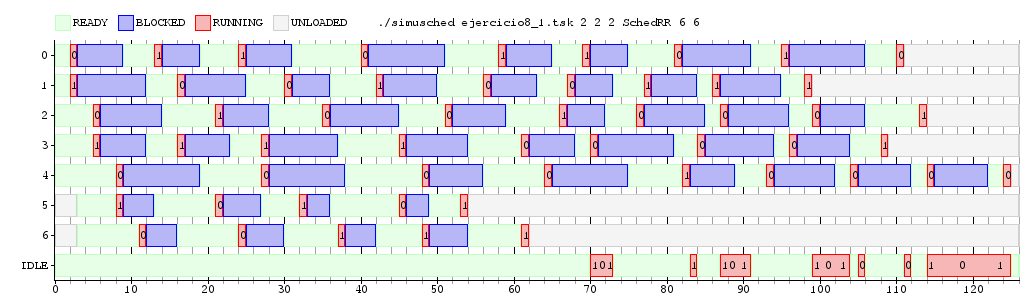
\includegraphics[scale=0.4]{graficos/ej8_RR_1.png}
\end{center}

La misma corrida sin migración de cores consume unos 20 ciclos menos de CPU para finalizar: \\

\begin{center}
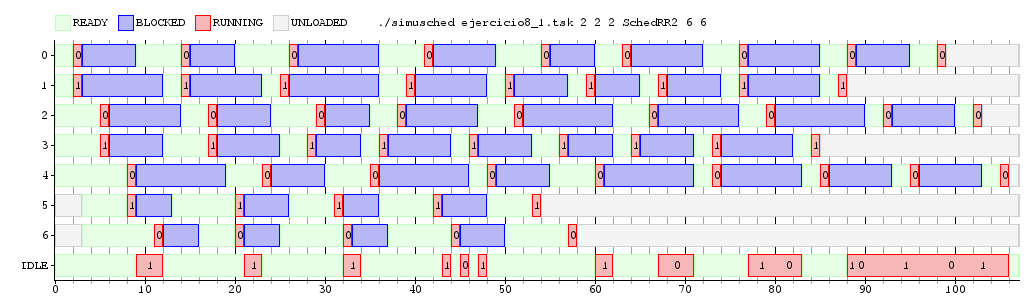
\includegraphics[scale=0.4]{graficos/ej8_RR2_1.png}
\end{center}

Existen casos en los que, en cambio, es conveniente migrar de cores. Consideremos un lote de tareas que se encuentran intercaladas entre tareas de larga duración y tareas cortas. El algoritmo de Round Robin sin migración de cores no sabe identificar este caso, por lo que quedarán acumuladas las tareas largas en un core, y las cortas en otro. Luego el segundo core quedará ocioso, mientras las otras tareas tienen que compartir el único core que tienen asignado hasta finalizar.\\

\noindent
Consideremos el siguiente lote:
\verbatiminput{graficos/corrida2_eje8.tsk}

Corrida con Round Robin con migración de cores: \\

\begin{center}
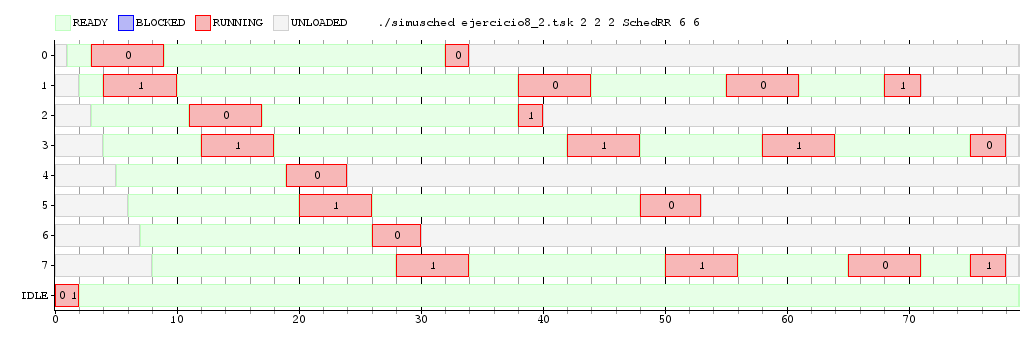
\includegraphics[scale=0.4]{graficos/ej8_RR_2.png}
\end{center}

Corrida con Round Robin sin migración de cores: \\

\begin{center}
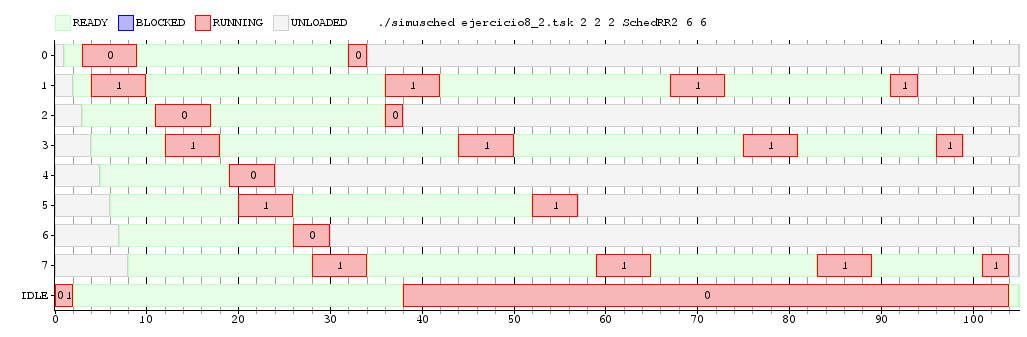
\includegraphics[scale=0.4]{graficos/ej8_RR2_2.png}
\end{center}

Notar que a partir del ciclo 38 el core 0 se encuentra ocioso, mientras aín quedan 4 tareas por completar en el core 1.\\


\subsection{Ejercicio 9}

Para mostrar con un ejemplo un caso que no sea factible para el scheduler RM y si lo sea para EDF nos basto el siguiente lote de 2 tareas periodicas:

Nota: Para simplicar el ejemplo consideramos en este caso despreciable el tiempo de cambio de contexto.
\\
\\
Lote:
\verbatiminput{graficos/lotes_ej9.tsk}

Produciendo los siguientes gráfico:

Para RM:

\begin{center}
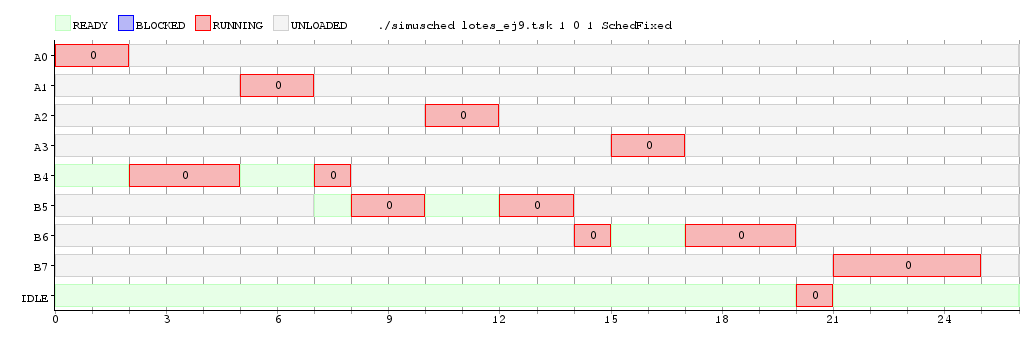
\includegraphics[scale=0.4]{graficos/eje9_fixed.png}
\end{center}

Para EDF:

\begin{center}
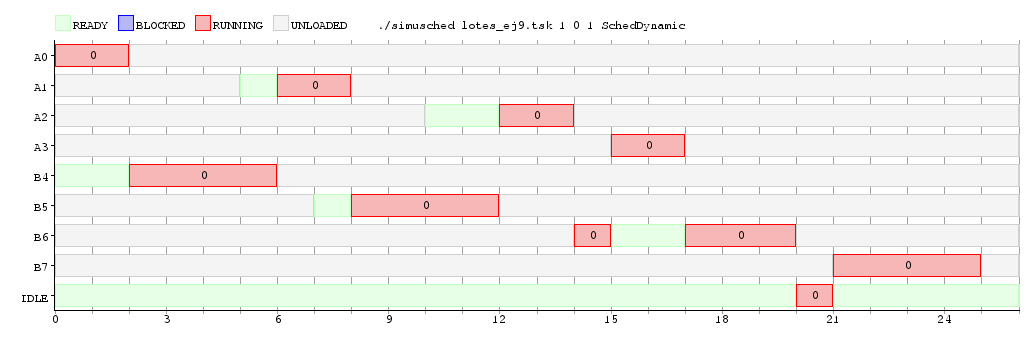
\includegraphics[scale=0.4]{graficos/eje9_dynamic.png}
\end{center}

La tarea de la familia A tiene un periodo menor que el de la familia B por lo cual según el scheduler RM tiene mayor prioridad asignada. Esta elección de priorizar a la familia A provoca un perjuicio en la familia B por lo que la familia B no puede cumplir su deadline en $T=7$ (Se produce un overflow).

En el caso del gráfico de EDF se puede observar que le da el CPU un poco más a la familia B por tener el deadline más próximo logrando evitar así el inclumplimiento del deadline (en $T=5$ deja esperando a la tarea de la familia A).

Algo interesante para destacar es que en este caso ambos scheduler ocuparon el mismo tiempo el CPU con trabajos, lo que cambia es que el scheduler RM a diferencia de EDF tiende a gastar más tiempo de computo en tareas de mayor prioridad dejandolo poco procesamiento a las de menor prioridad.

\subsection{Ejercicio 10}

En este caso encontramos un ejemplo en el cual las tareas son factibles tanto para RM como para EDF pero con un mejor uso de CPU por parte de EDF.

Nota: En este caso asignamos al cambio de contexto un costo 1.
\\
\\
Lote:
\verbatiminput{graficos/lotes_eje10.tsk}

Produciendo los siguientes gráficos:

Para RM:

\begin{center}
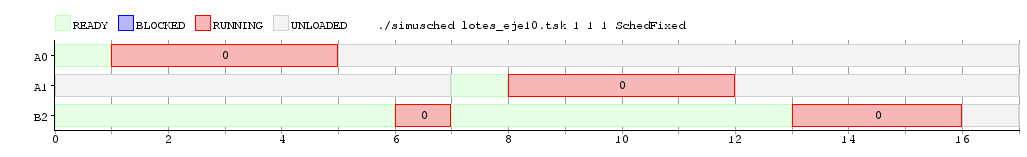
\includegraphics[scale=0.4]{graficos/eje10_Fixed.png}
\end{center}

Para EDF:

\begin{center}
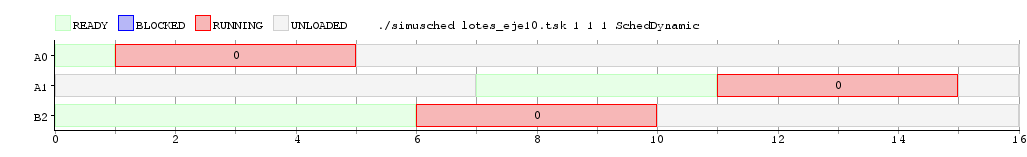
\includegraphics[scale=0.4]{graficos/eje10_Dynamic.png}
\end{center}

En este caso vemos que el scheduler RM necesita 1 cambio de contexto más que EDF lo que hace que el tiempo neto de procesamiento en tareas sea mayor en EDF (cambios de contexto con RM en T=\{0, 5, 7, 12\} mientras que EDF en T=\{0, 5, 10\}).

Intuitivamente se nos ocurre una conjetura para explicar este resultado, que sería que RM en general necesita más cambios de contexto porque toda tarea de menor prioridad es desalojada por las de mayor prioridad y como estas últimas tienen menor periodo (i.e. mayor frecuencia) la cantidad de desalojos es mayor.







%\section{Resultados}

\subsubsection*{Experimentos sobre el grado del polinomio interpolador}

\includegraphics[scale=0.5]{graficos/gradoPol.png}

Para el experimento sobre el grado del polinomio se corrieron todas las
instancias de las carpetas rectas, cuadráticas y cubicas provistas por la
cátedra.  Cada una de estas instancias se corrió para cada grado del polinomio,
por lo tanto se probaron 15 instancias por grado variando el grado de 1 a 8.

\begin{verbatim}
Cantidad de aciertos sobre 15 instancias
grado 1: 8 
grado 2: 10
grado 3: 13
grado 4: 13
grado 5: 13
grado 6: 10
grado 7: 9
grado 8: 8
\end{verbatim}


Los resultados se encuentran en el archivo visualizador/resultados/testGradoPol.out

\subsubsection*{Experimentos sobre el tamaño del historial}

\includegraphics[scale=0.5]{graficos/kPuntos.png}

Para el experimento del historial se utilizaron las siguientes instancias:

\begin{itemize}
  \item Curvas no atajas por el arquero anterior:
  \begin{itemize}
    \item cl.tiro
    \item c3.tiro
  \end{itemize}
 \item Curvas atajadas por el arquero anterior:
  \begin{itemize}
    \item c2.tiro
    \item r1.tiro
    \item cb1.tiro
  \end{itemize}
  \item Trayectos que no describen curvas exactas no probadas en el arquero anterior: 
  \begin{itemize}
   \item 1.tiro
   \item 2.tiro
   \item 3.tiro
   \item 4.tiro
   \end{itemize}
\end{itemize}

Se considera k=25 como el polinomio armado con todos los puntos de la
instancia, ya que ninguna instancia supera este numero de puntos.  Los
resultados son:

\begin{itemize}
\item Para K=25:
  \begin{itemize}
    \item Atajo: c2.tiro, r1.tiro, cb1.tiro,3.tiro,4.tiro
    \item No atajo: c1.tiro, c3.tiro, 1.tiro, 2.tiro
  \end{itemize}
\item Para K$\neq$25:
  \begin{itemize}
    \item Atajo: c2.tiro(exceptuando k=5), r1.tiro, cb1.tiro,3.tiro,4.tiro
    \item No atajo: c1.tiro, c3.tiro, 1.tiro, 2.tiro
  \end{itemize}
\end{itemize}

Los resultados se encuentran en el archivo visualizador/resultados/testK.out

Dado que las pruebas no mejoran ni empeoran el rendimiento de arquero al variar
este parámetro decidimos no limitar la cantidad de puntos tomados para nuestra
implementación final del robot.

\subsubsection*{Experimentos sobre las tácticas del arquero}

\includegraphics[scale=0.5]{graficos/tacticas.png}

En este grafico 0 significa sin tácticas, 1 significa solo táctica 1 y
2 solo táctica 2.

Para el experimento sobre las tácticas se utilizaron las instancias contenidas
en las carpetas fancy, instancia2 e instancias3.  Las parámetros se realizaron
con los parámetros $g=3$ y $k$ sin acotar.  Los resultados se encuentran en el
archivo visualizador/resultados/tac1ytac2.out


\includegraphics[scale=0.5]{graficos/grado_pol.png}

\includegraphics[scale=0.5]{graficos/grado_con_ruido30.png}
\includegraphics[scale=0.5]{graficos/grado_con_ruido70.png}

\includegraphics[scale=0.5]{graficos/cbp30_noRuido.png}
\includegraphics[scale=0.5]{graficos/cbp30_Ruido.png}
\includegraphics[scale=0.5]{graficos/cbp70_Ruido.png}
\includegraphics[scale=0.5]{graficos/cbp70_noRuido.png}
\includegraphics[scale=0.5]{graficos/rp70_noRuido.png}
\includegraphics[scale=0.5]{graficos/rp70_Ruido.png}


%\include{discusion}
\section{Conclusiones}

De este trabajo, nos quedo claro que para implementar un scheduler adecuado hay que fijarse en varios aspectos: \\

\begin{itemize}
	\item Como son las tareas a planificar (ej si son periodicas, si tienen deadlines, si tienden a bloquearse).
	\item Como es el hardware en el que van a correr (Si tiene uno o varios nucleos, costo de cambio de contexto, costo de migración de nucleos).
	\item Analizar el contexto o los requerimientos (Que peso tiene cada una de las diferentes métricas, tiempo de espera, eficicia de CPU, ..., etc).
\end{itemize}

%\bibliographystyle{plain}
%\bibliography{tp3}

\end{document}

